\documentclass[12pt, a4paper, oneside]{ctexart}
\usepackage{amsmath, amsthm, amssymb, bm, color, graphicx, geometry, mathrsfs,extarrows, braket, booktabs, array}
\usepackage[colorlinks,linkcolor=red,anchorcolor=blue,citecolor=blue,urlcolor=blue,menucolor=black]{hyperref}
\setmainfont{Times New Roman}  % 设置英文字体
\setsansfont{Calibri}
\setmonofont{Consolas}

\linespread{1.4}
%\geometry{left=2.54cm,right=2.54cm,top=3.18cm,bottom=3.18cm}
\geometry{left=1.84cm,right=1.84cm,top=2.18cm,bottom=2.18cm}
\newcounter{problem}
\newenvironment{problem}{\stepcounter{problem}\par\noindent\textbf{题目\arabic{problem}. }}{\smallskip\par}
\newenvironment{solution}{\par\noindent\textbf{解答. }}{\smallskip\par}
\newenvironment{note}{\par\noindent\textbf{注记. }}{\smallskip\par}

%%%% 图片相对路径 %%%%
\graphicspath{{figure/}} % 当前目录下的figure文件夹, {../figure/}则是父目录的figure文件夹

\everymath{\displaystyle} % 默认全部行间公式
\DeclareMathOperator*\uplim{\overline{lim}} % 定义上极限 \uplim_{}
\DeclareMathOperator*\lowlim{\underline{lim}} % 定义下极限 \lowlim_{}
\let\leq=\leqslant % 将全部leq变为leqslant
\let\geq=\geqslant % geq同理

%%%% 一些宏定义 %%%%
\def\bd{\boldsymbol}        % 加粗(向量) boldsymbol
\def\disp{\displaystyle}    % 使用行间公式 displaystyle(默认)
\def\tsty{\textstyle}       % 使用行内公式 textstyle
\def\sign{\text{sign}}      % sign function
\def\wtd{\widetilde}        % 宽波浪线 widetilde
\def\R{\mathbb{R}}          % Real number
\def\N{\mathbb{N}}          % Natural number
\def\Z{\mathbb{Z}}          % Integer number
\def\C{\mathbb{C}}          % Complex number
\def\d{\mathrm{d}}          % differential operator
\def\e{\mathrm{e}}          % Euler's number
\def\i{\mathrm{i}}          % imaginary number
\def\re{\mathrm{Re}}        % Real part
\def\im{\mathrm{Im}}        % Imaginary part
\def\res{\mathrm{Res}}      % Residue
\def\L{\mathcal{L}}         % Loss function
\def\wdh{\widehat}          % 宽帽子 widehat
\def\ol{\overline}          % 上横线 overline
\def\ul{\underline}         % 下横线 underline
\def\add{\vspace{1ex}}      % 增加行间距
\def\del{\vspace{-3.5ex}}   % 减少行间距

%%%% 定理类环境的定义 %%%%
\newtheorem{theorem}{定理}

%%%% 基本信息 %%%%%
\newcommand{\RQ}{\today} % 日期
\newcommand{\km}{偏微分方程} % 科目
\newcommand{\bj}{强基数学002} % 班级
\newcommand{\xm}{吴天阳} % 姓名
\newcommand{\xh}{2204210460} % 学号

\begin{document}

%\pagestyle{empty}
\pagestyle{plain}
\vspace*{-15ex}
\centerline{\begin{tabular}{*5{c}}
    \parbox[t]{0.25\linewidth}{\begin{center}\textbf{日期}\\ \large \textcolor{blue}{\RQ}\end{center}} 
    & \parbox[t]{0.2\linewidth}{\begin{center}\textbf{科目}\\ \large \textcolor{blue}{\km}\end{center}}
    & \parbox[t]{0.2\linewidth}{\begin{center}\textbf{班级}\\ \large \textcolor{blue}{\bj}\end{center}}
    & \parbox[t]{0.1\linewidth}{\begin{center}\textbf{姓名}\\ \large \textcolor{blue}{\xm}\end{center}}
    & \parbox[t]{0.15\linewidth}{\begin{center}\textbf{学号}\\ \large \textcolor{blue}{\xh}\end{center}} \\ \hline
\end{tabular}}
\vspace*{4ex}

% 正文部分
\begin{theorem}[Gauss-Green公式]
    设$\Omega\in\R^n$为有界开集,且$\partial\Omega\in C^1$,若$U=(u_1,\cdots,u_n)^T:\bar{\Omega}\to\R^n$且$u\in C^1(\Omega)\cap C(\bar{\Omega})$,则
    \begin{equation*}
        \int_{\Omega}\nabla\cdot U\,\d x = \int_{\partial\Omega}U\cdot \bd{n}\,\d s,
    \end{equation*}
    其中$\bd{n}$为$\partial \Omega$的单位外法向.
\end{theorem}
\begin{problem}
    利用Gauss-Green公式证明:

    (1). 若$u, v\in C^1(\Omega)\cap C(\bar{\Omega})$,则
    \begin{equation*}
        \int_{\Omega}u_{x_i}v\,\d x = -\int_{\Omega}uv_{x_i}\,\d x+\int_{\partial \Omega}uvn_i\,\d s.
    \end{equation*}

    (2). 若$u\in C^2(\Omega)\cap C^1(\bar{\Omega})$,则
    \begin{equation*}
        \int_{\Omega}\Delta u\,\d x=\int_{\partial \Omega}\frac{\partial u}{\partial \bd{n}}\,\d s,
    \end{equation*}
    其中$\Delta u=\nabla\cdot(\nabla u) = \sum_{i=1}^n\frac{\partial^2 u}{\partial x_i^2},\ \frac{\partial u}{\partial \bd{n}}=\nabla u\cdot \bd{n}$.\add

    (3). 若$u, v\in C^2(\Omega)\cap C^1(\bar{\Omega})$,则
    \begin{equation*}
        \int_{\Omega}\nabla u\cdot \nabla v\,\d x=-\int_{\Omega} u\nabla v\,\d x+\int{\partial \Omega}u\frac{\partial v}{\partial \bd{n}}\,\d s.
    \end{equation*}\del

    (4). 若$u,v\in C^2(\Omega)\cap C^1(\bar{\Omega})$,则
    \begin{equation*}
        \int_{\Omega}(u\Delta v-v\Delta u)\,\d x=\int_{\partial \Omega}\left(u\frac{\partial v}{\partial\bd{n}}-v\frac{\partial u}{\partial \bd{n}}\right)\,\d s.
    \end{equation*}
\end{problem}
\begin{proof}
    (1). 令$U = (0,\cdots, 0, uv, 0,\cdots, 0)^T$,即$U_j = \begin{cases}uv,&\quad j=i,\\ 0,&\quad j\neq i.\end{cases}$ 则
    \begin{equation*}
        \begin{aligned}
            \int_{\Omega}\nabla\cdot U\,\d x =&\ \int_{\Omega}\frac{\partial uv}{\partial x_i}\,\d x=\int_{\Omega}u_{x_i}v\,\d x+\int_{\Omega}uv_{x_{i}}\,\d x\\
            \xlongequal{\text{Gauss-Green}}&\ \int_{\partial \Omega}U\cdot \bd{n}\,\d s=\int_{\partial \Omega}uvn_i\,\d s\\
        \end{aligned}\Rightarrow
        \int_{\Omega}u_{x_i}v\,\d x=-\int_{\Omega}uv_{x_i}\,\d x+\int_{\partial\Omega}uvn_i\,\d s.
    \end{equation*}

    (2). \begin{equation*}
        \int_{\Omega}\Delta u\,\d x=\int_{\Omega}\nabla\cdot(\nabla u)\,\d x \xlongequal{\text{Gauss-Green}}\int_{\partial \Omega}\nabla u\cdot \bd{n}\,\d s = \int_{\partial \Omega}\frac{\partial u}{\partial \bd{n}}\,\d s.
    \end{equation*}

    (3). 由$(1)$知,令$v=\frac{\partial v}{\partial x_i}$,可得
    \begin{equation*}
        \int_{\Omega}\frac{\partial u}{\partial x_i}\frac{\partial v}{\partial x_i}\,\d x =-\int_{\Omega}u\frac{\partial^2 v}{\partial x_i^2}\,\d x+\int_{\partial \Omega}u\frac{\partial v}{\partial x_i}n_i\,\d s,\quad(i=1,2,\cdots, n),
    \end{equation*}
    对上式左右两端同时对$i=1,2,\cdots, n$求和可得
    \begin{equation*}
        \int_{\Omega}\nabla u\cdot \nabla v\,\d x = -\int_{\Omega}u\Delta v\,\d x+\int_{\partial \Omega}u\frac{\partial v}{\partial \bd{n}}\,\d s.
    \end{equation*}

    (4). 由$(3)$知,交换$u, v$可得
    \begin{equation*}
        \int_{\Omega}\nabla u\cdot \nabla v\,\d x = -\int_{\Omega}u\Delta v\,\d x+\int_{\partial \Omega}u\frac{\partial v}{\partial \bd{n}}\,\d s=-\int_{\Omega}v\Delta u\,\d x+\int_{\partial \Omega}v\frac{\partial u}{\partial \bd{n}}\,\d s,
    \end{equation*}
    则
    \begin{equation*}
        \int_{\Omega}(u\Delta v-v\Delta u)\,\d x =\int_{\partial \Omega}\left(u\frac{\partial v}{\partial \bd{n}}-v\frac{\partial u}{\partial \bd{n}}\right)\,\d s.
    \end{equation*}
\end{proof}
\begin{problem}
    将下列方程化为标准型:
    \begin{align*}
        (1)&\ \sum_{i=1}^nu_{x_ix_i}+\sum_{1\leq i<j\leq n}u_{x_ix_j}=0,\\
        (2)&\ u_{xx}+2u_{xy}+2u_{yy}=0.
    \end{align*}
\end{problem}
\begin{solution}
    (1). 该方程的系数矩阵为$A = \left[\begin{matrix}
        1&1/2&\cdots&1/2\\
        1/2&1&\cdots&1/2\\
        \vdots&\vdots&\ddots&\vdots\\
        1/2&1/2&\cdots&1
    \end{matrix}\right]$,则$A$的有$n-1$重特征值为$\lambda_{1,2,\cdots,n-1}=\frac{1}{2}$,$\lambda_n = \frac{n+1}{2}$,于是该方程为\textbf{椭圆形},通过变量代换
    \begin{equation*}
        \nabla v = \left[\begin{matrix}
            \frac{1}{\sqrt{2}}&\frac{1}{\sqrt{6}}&\cdots&\frac{1}{\sqrt{n(n-1)}}&\frac{1}{\sqrt{n}}\\
            -\frac{1}{\sqrt{2}}&\frac{1}{\sqrt{6}}&\cdots&\frac{1}{\sqrt{n(n-1)}}&\frac{1}{\sqrt{n}}\\
            0&-\frac{2}{\sqrt{6}}&\ddots&\vdots&\vdots\\
            \vdots&\vdots&\ddots&\frac{1}{\sqrt{n(n-1)}}&\frac{1}{\sqrt{n}}\\
            0&0&\cdots&-\frac{(n-1)}{\sqrt{n(n-1)}}&\frac{1}{\sqrt{n}}
        \end{matrix}\right]\nabla u
    \end{equation*}
    可得标准型为$\sum_{i=1}^n\lambda_iv_{x_ix_i}=0$.

    (2). 该方程的系数矩阵为$A = \left[\begin{matrix}
        1&1\\1&2
    \end{matrix}\right]$,则$A$的特征值为$\lambda_{1,2}=\frac{3\pm\sqrt{5}}{2}$,则该方程为\textbf{椭圆形},通过变量代换
    \begin{equation*}
        \nabla v = \left[\begin{matrix}
            \sqrt{\frac{5+\sqrt{5}}{10}}&\sqrt{\frac{5-\sqrt{5}}{10}}\\
            -\sqrt{\frac{5-\sqrt{5}}{10}}&\sqrt{\frac{5+\sqrt{5}}{10}}
        \end{matrix}\ \right]\nabla u
    \end{equation*}
    可得标准型为$\sum_{i=1}^n\lambda_iv_{x_ix_i}=0$.
\end{solution}
\begin{problem}
    设\begin{equation*}
        J(v) = \frac{1}{2}\int_{\Omega}(|\nabla v|^2+v^2)\,\d x+\frac{1}{2}\int_{\partial \Omega}\alpha(x)v^2\,\d s-\int_{\Omega}fv\,\d x-\int_{\partial \Omega}gv\,\d s,
    \end{equation*}
    其中$\alpha(x) \geq 0$. 考虑一下三个问题:
    
    问题I(变分问题):求$u\in M=C^1(\bar{\Omega})$,使得
    \begin{equation*}
        J(u)=\min_{v\in M}J(v).
    \end{equation*}

    问题II:求$u\in M=C^1(\bar{\Omega})$,使得它对于任意$v\in M$,都满足
    \begin{equation*}
        \int_{\Omega}(\nabla u\cdot \nabla v+u\cdot v-fv)\,\d x+\int_{\partial \Omega}(\alpha(x)uv-gv)\,\d s=0.
    \end{equation*}

    问题III(第三边值问题):求$u\in C^2(\Omega)\cap C^1(\bar{\Omega})$,满足以下边值问题
    \begin{equation*}
        \begin{cases}
            -\Delta u+u=f,&\quad x\in\Omega,\\
            \frac{\partial u}{\partial \vec{n}}+\alpha(x)u=g,&\quad x\in\partial\Omega.
        \end{cases}
    \end{equation*}

    (1) 证明问题I与问题II等价.

    (2) 当$u\in C^2(\Omega)\cap C^1(\bar{\Omega})$时,证明问题I、II、III等价.
\end{problem}
\begin{solution}
    (1) $\forall v\in M$,$\forall \varepsilon > 0$,则$u+\varepsilon v\in M$,记
    \begin{equation*}
        j(\varepsilon) = J(u+\varepsilon v),
    \end{equation*}
    则
    \begin{equation*}
        j'(\varepsilon) = \int_{\Omega}((u_x+\varepsilon v_x)v_x+(u_y+\varepsilon v_y)v_y+(u+\varepsilon v) v)\,\d x + \int_{\partial \Omega}\alpha(x)(u+\varepsilon v)v\,\d s-\int_{\Omega}fv\,\d x-\int_{\partial \Omega}gv\,\d s.
    \end{equation*}
    问题I的必要性条件为$j'(0) = 0$,即
    \begin{align}
        \notag j'(0) =&\ \int_{\Omega}(u_xv_x+u_yv_y+uv)\,\d x+\int_{\partial \Omega}\alpha(x)uv\,\d s - \int_{\Omega}fv\,\d x-\int_{\partial \Omega}gv\,\d s\\
        =&\ \int_{\Omega}(\nabla u\cdot \nabla v+u v-fv)\,\d x+\int_{\partial \Omega}(\alpha(x)uv-gv)\,\d s=0.
    \end{align}
    由于
    \begin{equation*}
        j''(\varepsilon) = \int_{\Omega}(v_x^2+v_y^2+v^2)\,\d x+\int_{\partial \Omega}\alpha(x)v^2\,\d s\geq 0.
    \end{equation*}
    说明$(1)$式为问题I的充要条件,则问题I与问题II等价.

    (2) 由于$u\in C^2(\Omega)\cap C^1(\bar{\Omega})$,由Guass-Green公式可知
    \begin{equation*}
        \int_{\Omega}\nabla u\cdot \nabla v\,\d x = -\int_{\Omega}\Delta u\cdot v\,\d x+\int_{\partial \Omega}v\frac{\partial u}{\partial\vec{n}}\,\d s,
    \end{equation*}
    于是$(1)$式等价于
    \begin{equation*}
        \int_{\Omega}(u-\Delta u-f)v\,\d x+\int_{\partial \Omega}\left(\frac{\partial u}{\partial \vec{n}}+\alpha(x)u-g\right)v\,\d s=0,
    \end{equation*}
    取$v\in C_0^{\infty}(\Omega)$,由\textbf{引理2.1}可知
    \begin{equation*}
        \begin{cases}
            u = \Delta u  +f,&\quad x\in\Omega,\\
            \frac{\partial u}{\partial \vec{n}}+\alpha(x)u=g,&\quad x\in\partial\Omega.
        \end{cases}
    \end{equation*}
    综上,问题I与问题III等价,由(1)问可知,问题I、II、III等价.
\end{solution}
\begin{problem}
    (1) 证明在自变量代换
    \begin{equation*}
        \begin{cases}
            \xi = x-at,\\
            \eta = x + at
        \end{cases}
    \end{equation*}
    下,波动方程$u_{tt}-a^2u_{xx} = 0$具有的形式
    \begin{equation*}
        u_{\xi\eta}=0,
    \end{equation*}
    并由此求出波动方程的通解.

    (2) 证明在自变量代换
    \begin{equation*}
        \begin{cases}
            \xi = x-\alpha t,\\
            \tau = t
        \end{cases}
    \end{equation*}
    下,方程$u_t+\alpha u_x=a^2 u_{xx}$具有的形式
    \begin{equation*}
        u_{\tau} = a^2u_{\xi\xi}.
    \end{equation*}
\end{problem}
\begin{solution}
    (1) 由于$\xi_t = -a,\ \xi_x = 1,\ \eta_t = a,\ \eta_x =1$,则
    \begin{align*}
        u_{tt} - a^2u_{xx} = u_{\xi\eta}\cdot \xi_t\eta_t - a^2u_{\xi\eta}\cdot \xi_x\eta_x = -2a^2u_{\xi\eta} = 0
    \end{align*}
    则$u_{\xi\eta} = 0$. 对$\xi$进行积分可得$u_{\eta} = c+f(\eta)$,对$\eta$进行积分可得
    \begin{equation*}
        u=c\eta+\int f(\eta)\,\d \eta+f_2(\xi),
    \end{equation*}
    记$f_1(\eta) = c\eta+\int f(\eta)\,\d \eta$,则
    \begin{equation*}
        u(x, y) = f_1(x+at) + f_2(x-at).
    \end{equation*}
    其中$f_1,f_2$为任意的标量函数.

    (2) 由于$\xi_x = 1,\ \tau_x = 0,\ \tau_t = 1$,则
    \begin{align*}
        u_t+\alpha u_x =&\ u_\tau\tau_t + \alpha u_\tau\tau_x = u_\tau,\\
        \alpha^2u_{xx} =&\ \alpha^2u_{\xi\xi}(\xi_x)^2 = \alpha^2 u_{\xi\xi},
    \end{align*}
    所以原方程等价于$u_\tau = \alpha^2 u_{\xi\xi}$.
\end{solution}
\begin{problem}
    若$u$是Laplace方程$\Delta u=0$的解,如果$u(x)$只是向径$r=|x|$的函数,即$u(x) = \tilde{u}(r)$,试写出$\tilde{u}(r)$适合的常微分方程.
\end{problem}
\begin{solution}
    设$r=\sqrt{x_1^2+\cdots+x_n^2}$,则
    \begin{align*}
        \frac{\partial}{\partial x_i} =&\ \frac{\partial r}{\partial x_i}\,\frac{\partial}{\partial r} = \frac{x_i}{r}\,\frac{\partial}{\partial r},\\
        \frac{\partial^2}{\partial x_i^2} =&\ \frac{\partial^2}{\partial x_i^2}(\frac{x_i}{r}\frac{\partial}{\partial r}) = \frac{\partial^2}{\partial x_i^2}(\frac{x_i}{r})\frac{\partial}{\partial r}+(\frac{x_i}{r})^2\frac{\partial^2}{\partial r^2}= \frac{r^2-x_i^2}{r^3}\,\frac{\partial}{\partial r}+\frac{x_i^2}{r^2}\frac{\partial^2}{\partial r^2}.
    \end{align*}
    所以
    \begin{equation*}
        \Delta u = \sum_{i=1}^n\frac{\partial^2}{\partial x_i^2}u = \left(\frac{nr^2-r^2}{r^3}\,\frac{\partial}{\partial r}+\frac{r^2}{r^2}\,\frac{\partial^2}{\partial r^2}\right)u = \frac{\partial^2u}{\partial r^2}+\frac{n-1}{r}\frac{\partial u}{\partial r}.
    \end{equation*}
\end{solution}

% 下面给一些功能的写法
\iffalse
% 图片模板
\centerline{
    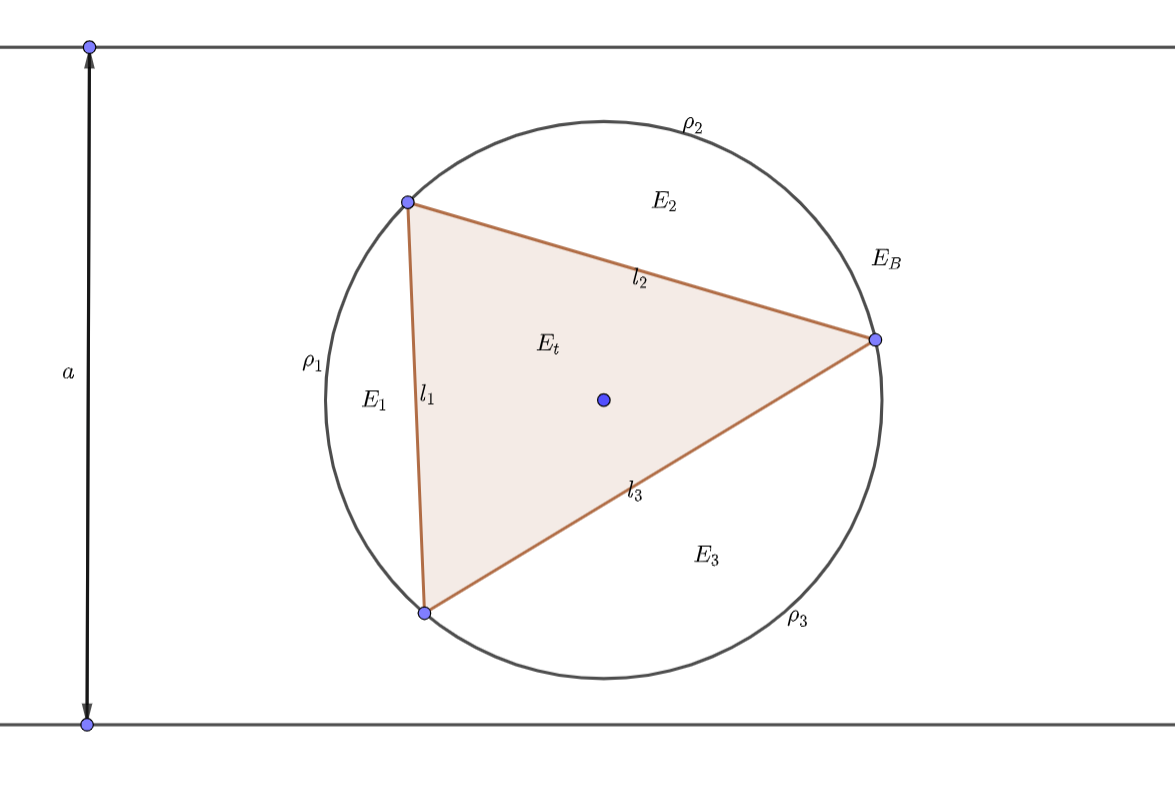
\includegraphics[width=0.8\textwidth]{figure.png}
}
% 表格模板
\renewcommand\arraystretch{0.8} % 设置表格高度为原来的0.8倍
\begin{table}[!htbp] % table标准
    \centering % 表格居中
    \begin{tabular}{p{1cm}<{\centering}p{1cm}<{\centering}p{3cm}<{\centering}p{5cm}<{\centering}} % 设置表格宽度
    %\begin{tabular}{cccc}
        \toprule
        $x_i$ & $f[x_1]$ & $f[x_i,x_{i+1}]$ & $f[x_i,x_{i+1},x_{i+2}]$ \\
        \midrule
        $x_0$ & $f(x_0)$ &                  &                          \\
        $x_0$ & $f(x_0)$ & $f'(x_0)$        &                          \\
        $x_0$ & $f(x_1)$ & $\frac{f(x_1)-f(x_0)}{x_1-x_0}$ & $\frac{f(x_1)-f(x_0)}{(x_1-x_0)^2}-\frac{f'(x_0)}{x_1-x_0}$\\
        \bottomrule
    \end{tabular}
\end{table}

\def\Log{\text{Log}} % 一个简单的宏定义
$\Log$ % 调用方法
\fi

\end{document}